\documentclass{article}
\usepackage{graphicx}
\usepackage{ragged2e}
\usepackage{geometry}
\title{Experimentation}
\author{Vigneswaran Chandrasekaran}
\date{10-11-2019}

\begin{document}
\flushleft{\huge{\textbf{Experimental Setup and Discussions}}}
\section{Experimental Setup}
\justify
In order to examine the effectiveness of the proposed \textit{unsupervised bin wise pre-training}
model in terms of both as a Optimizer and Regularizer, three benchmark datasets were used:
(i)MNIST handwritten digits dataset (ii) Zalando's article images dataset (Fashion MNIST) and (iii) University of Bern EEG dataset.

Evaluating on different characteristic datasets would help to estimate the benefit gained and ubiquitous nature of the proposed work. To make the experimentation process simple and efficient, models were designed with minimal number of architectural elements to enforce parsimony[].For all three datasets, Cross entropy loss was employed as the objective function, Rectified Linear Units (ReLUs) was set as activation function and Adam optimizer was applied. The models were implemented in Python3 using PyTorch library. In addition, NumPy and Matplotlib were used to perform matrix operations and plotting respectively.All the experimentation were carried out in the machine with 6 GB of Primary Memory, Intel i3 dual core CPU with 1.7 GHz and 64-bit Debian operating system.

\subsection{MNIST dataset}
The MNIST dataset consists of handwritten digits, which are widely preferred
by the researchers to evaluate their proposed models. The dataset comprises of 70,000
handwritten digit images, out of which 60,000 and 10,000 images were used for training
(TR$_{D1}$) and testing ( TE$_{D1}$ ) respectively. The training dataset ( TR$_{D1}$ ) was sub-divided into
training dataset ( T$_{D1}$ ) and validation dataset ( V$_{D1}$ ) in the ratio 80:20 (48,000:12,000). DNN
was configured with an input layer consisting of 784 (28 x 28 pixels) input neurons, five
hidden layers comprising 1024, 200, 20, 20, 20 neurons in each layer respectively and an
output layer with 10 output neurons which corresponds the class labels of the MNIST dataset.

\subsection{Zalando's article images dataset}
Zalando's article images dataset consists of 60,000 training and 10,000 testing examples, with each example represents a $28x28$ grayscale image associated with a class from 10 different articles of clothing classes. Due to its high similarity with original MNIST dataset, it is popularly known as Fashion MNIST. As with MNIST dataset, the TR$_{D2}$ was divided into T$_{D2}$ and V$_{D2}$ in 80:20 ratio, and DNN model was configured with hidden layers of dimension 1024, 200, 20, 20, 20 and output layer of size 10.

\subsection{University of Bern EEG dataset}
University of Bern-Barcelona EEG dataset comprises of EEG recordings from five epileptic patients using intracranial method[$CitationReq$]. During data acquisition the sampling rate was set either 512 or 1024 Hz and later down-sampled to 512Hz. Dataset consists of 7500 samples with equally balanced focal and non-focal types which in turn each sample consists of 10,240 data points. The reason behind for choosing a dataset of physiological signals for evaluating the proposed work is because of their extremely complex and vulnerable to noise behavior.  
The dominance of DNNs over interpreting physiological signals is still not as expected and a much amount of research is devoted in this field [https://www.sciencedirect.com/science/article/pii/S0169260718301226]. As a common approach of EEG preprocessing, the signals were decomposed using Daubechies10 basis wavelet function [Scopus paper citing]  and entropy features (comprising of Sample, Shannon, Permutation and Multiscale entropies) were extracted. The datset was splitted into T$_{D3}$, V$_{D3}$ and TE$_{D3}$ in 60:30:10 ratio, and DNN architecture was designed with hidden layers of size 200, 150, 100, 20 and the output layer with size 2.

\section{Discussions}
The goal of this research article is to develop a parochial pre-training model which
initializes near optimal parameters by forming bins based on the MI between the input
data and the neuron activations. Further, the number of bins was selected using partial
information decomposition and the parameters were updated using the novel weight
update rule during pre-training. This way of pre-training ensures the high possibility of
reaching the near global optimal position. To show the supremacy of the proposed model
in terms of stability, convergence rate, the comparisons were made with state-of-the-art
weight initialization methods and pre-training techniques.

\subsection{Comparison with other Weight Initialization methods}
To check how effective the parameters obtained from unsupervised bin-wise pre-training
model can effectively locate the model near to the potential local minima and results to
faster convergence, the proposed work was compared with various Weight Initialization
methods. Well-known and effective Weight initialization methods including Xavier [43],
Kaiming [44] and Orthogonal methods [42] were taken into account for comparison. All the weight initialization methods were configured with default parameter values as mentioned in Pytorch's torch.nn.init module to make the results obtain more reliable.
\\
\vspace{4cm} 
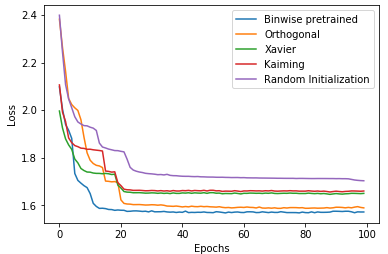
\includegraphics[width= 7cm, height=5cm]{fig1.png}
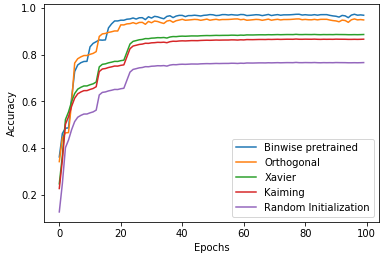
\includegraphics[width= 7cm, height=5cm]{fig2.png}
\\
Fig 7(a) \& Fig 7(b) shows the validation loss and Validation accuracy of various Weight Initialization methods for MNIST dataset respectively
\\
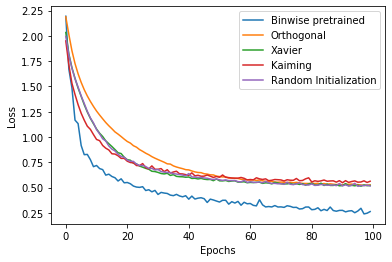
\includegraphics[width= 7cm, height=5cm]{fig5.png}
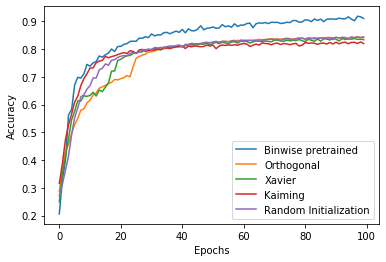
\includegraphics[width= 7cm, height=5cm]{fig6.png}
\\
Fig 8(a) \& Fig 8(b) depicts the validation loss and Validation accuracy of various Weight Initialization methods for Fashion MNIST dataset respectively
\\
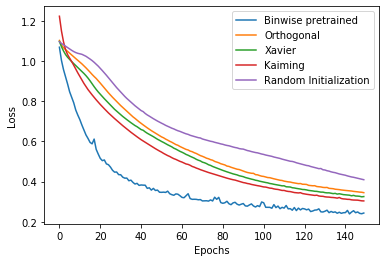
\includegraphics[width= 7cm, height=5cm]{fig3.png}
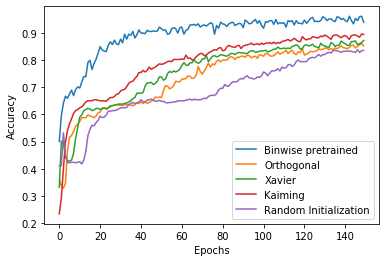
\includegraphics[width= 7cm, height=5cm]{fig4.png}
Fig 9(a) \& Fig 9(b) plots the validation loss and Validation accuracy of various Weight Initialization methods for University of Bern EEG dataset respectively
\\
Figure 7, 8 and 9 shows clear dominance of the proposed binwise pretraining method.
\\

\subsection{Comparison with other Pre-training techniques}
The proposed bin-wise pre-training model was compared with the existing pre-training
models: Stacked Autoencoders and Supervised Greedy layer-wise pre-training model.
Stacked Autoencoder was configured with three stacks of encoder-decoder, whereas
Supervised Greedy layer-wise pre-training model was shaped with six layers added
sequentially.
\\
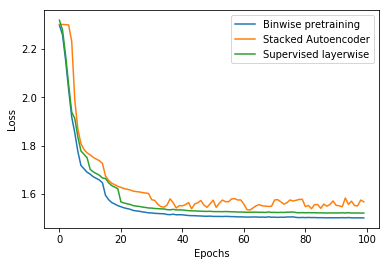
\includegraphics[width= 7cm, height=5cm]{fig7.png}
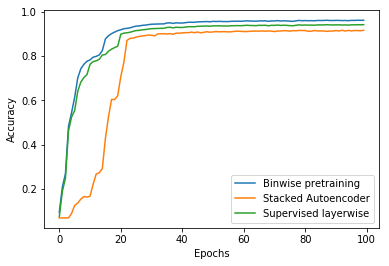
\includegraphics[width= 7cm, height=5cm]{fig8.png}
\\
Fig 10(a) \& Fig 10(b) shows the validation loss and Validation accuracy of Pretraining methods for MNIST dataset respectively
\\
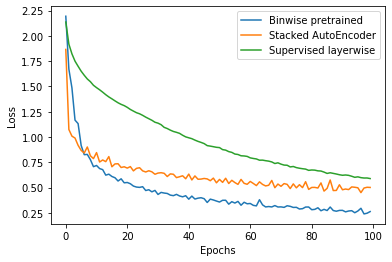
\includegraphics[width= 7cm, height=5cm]{fig9.png}
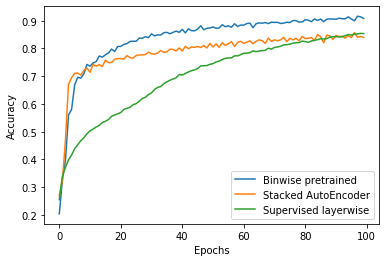
\includegraphics[width= 7cm, height=5cm]{fig10.png}
\\
Fig 11(a) \& Fig 11(b) depicts the validation loss and Validation accuracy of Pretraining methods for Fashion MNIST dataset respectively
\\
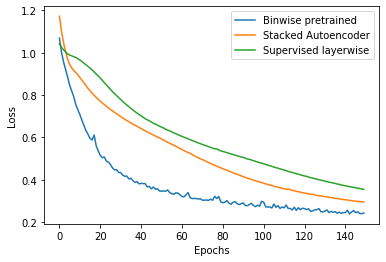
\includegraphics[width= 7cm, height=5cm]{fig11.png}
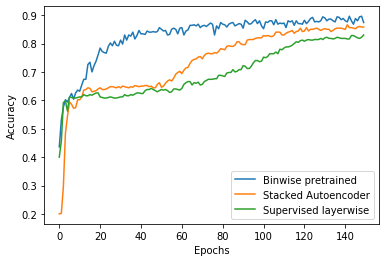
\includegraphics[width= 7cm, height=5cm]{fig12.png}
Fig 12(a) \& Fig 12(b) plots the validation loss and Validation accuracy of various Pretraining methods for University of Bern EEG dataset respectively
\begin{table}
	\begin{tabular}{c|c|c|c|c|c|c|}
		\cline{2-7}
		& \multicolumn{2}{c|}{\textbf{MNIST}} & \multicolumn{2}{c|}{\textbf{Fashion MNIST}} & \multicolumn{2}{c|}{\textbf{University of Bern EEG}} \\ \hline
		\multicolumn{1}{|c|}{\textbf{Methods}}              & Sensitivity      & Specificity      & Sensitivity          & Specificity          & Sensitivity               & Specificity              \\ \hline
		\multicolumn{1}{|c|}{\textbf{Stacked Autoencoders}} & 0.899            & 0.891            & 0.796                & 0.804                & 0.839                     & 0.837                    \\ \hline
		\multicolumn{1}{|c|}{\textbf{Supervised layerwise}} & 0.943            & 0.944            & 0.807                & 0.818                & 0.786                     & 0.782                    \\ \hline
		\multicolumn{1}{|c|}{\textbf{Binwise pretrained}}   & \textbf{0.964}   & \textbf{0.966}   & \textbf{0.915}       & \textbf{0.922}       & \textbf{0.936}            & \textbf{0.945}           \\ \hline
	\end{tabular}
\end{table}
\begin{table}[]
	\begin{tabular}{c|c|c|c|c|c|c|}
		\cline{2-7}
		& \multicolumn{2}{c|}{\textbf{MNIST}} & \multicolumn{2}{c|}{\textbf{Fashion MNIST}} & \multicolumn{2}{c|}{\textbf{University of Bern EEG}} \\ \hline
		\multicolumn{1}{|c|}{\textbf{Methods}}            & Sensitivity      & Specificity      & Sensitivity          & Specificity          & Sensitivity               & Specificity              \\ \hline
		\multicolumn{1}{|c|}{\textbf{Orthogonal}}         & 0.938            & 0.923            & 0.791                & 0.803                & 0.826                     & 0.833                    \\ \hline
		\multicolumn{1}{|c|}{\textbf{Xavier}}             & 0.817            & 0.823            & 0.813                & 0.812                & 0.782                     & 0.787                    \\ \hline
		\multicolumn{1}{|c|}{\textbf{Kaiming}}            & 0.795            & 0.802            & 0.786                & 0.775                & 0.834                     & 0.829                    \\ \hline
		\multicolumn{1}{|c|}{\textbf{Binwise pretrained}} & \textbf{0.964}   & \textbf{0.966}   & \textbf{0.915}       & \textbf{0.922}       & \textbf{0.936}            & \textbf{0.945}           \\ \hline
	\end{tabular}
\end{table}
\\
\subsection{Regularization Capability}
To evaluate the performance of the proposed work in Regularization perspective, the
distribution of randomly initialized weights and weights after bin-wise pre-training
were recorded and the change imbibed on them due to bin-wise pre-training were
analysed. It was inferred that the weight boundaries were maintained within 0.04 and
the variance of both the distribution remains the same throughout the pre-training
process which confirms that the proposed model behaves as a good regularizer. Fig. 13.
shows the comparison of distribution of randomly initialized weights and pre-trained
weights. Fig. 14. depicts the pattern of weight updation during pre-training process and
it was inferred that the new weights obtained had the desirable distribution, thus
making the Deep Learning model simple with better Generalization behaviour along
with less susceptible to overfitting and Vanishing or Exploding gradient problems.
\\
\\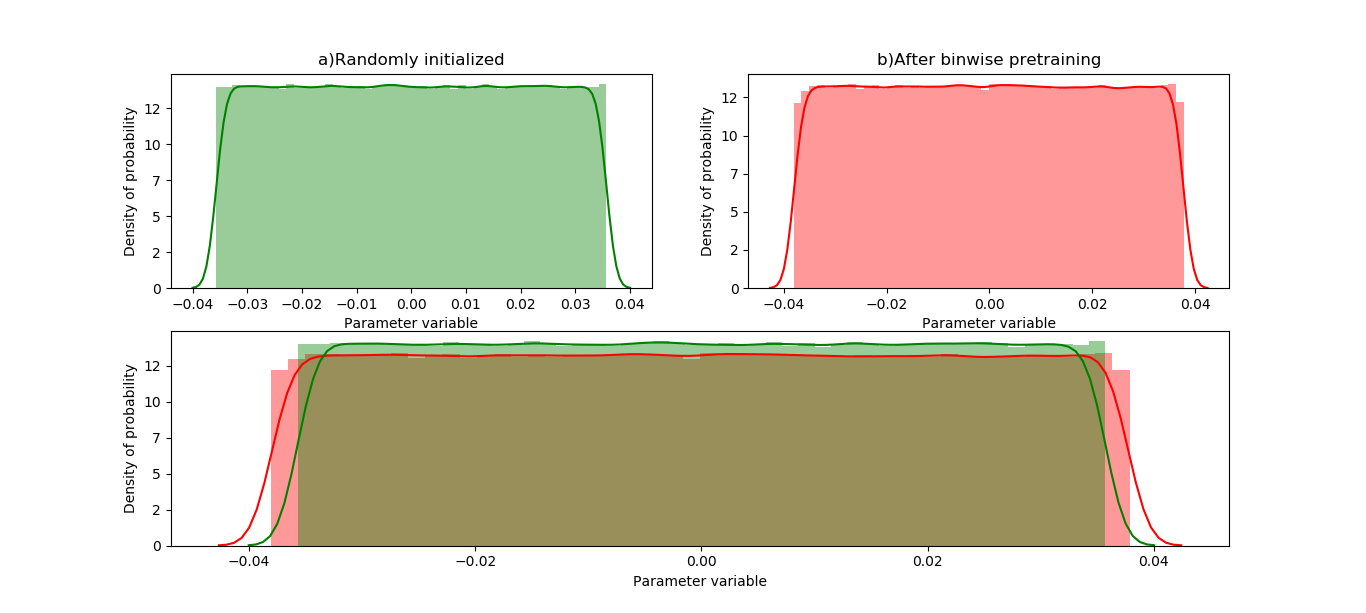
\includegraphics[width= 15cm, height=8cm]{fig13.png}
\\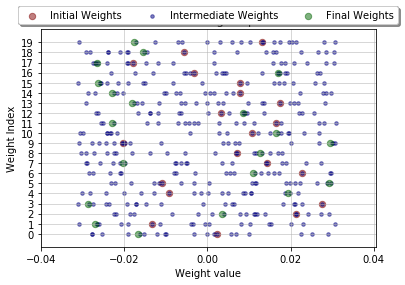
\includegraphics[width= 15cm, height=8cm]{fig14.png}
\\
Fig. 14. Weight updation pattern of randomly selected twenty weights for twenty
iterations during pre-training process.
\\
\subsection{Convergence Rate}
Rate of convergence is an important metric that measures the ability of the model to
converge in better minima with reasonable amount of time. From Fig. 7, 8 \& 9 it has
been inferred that the rate of convergence for all the existing approaches were mostly
similar at the beginning and as the iteration proceeded the proposed unsupervised bin-
wise pre-training model converges earlier than others. Selecting appropriate number of
bins using Partial Information Decomposition alters the degree of change and directly
influences the convergence rate. Fig. 15. shows the increase in Mutual Information
between Neuron’s output ( ) and Input data ( ) as the iterations were proceeded.
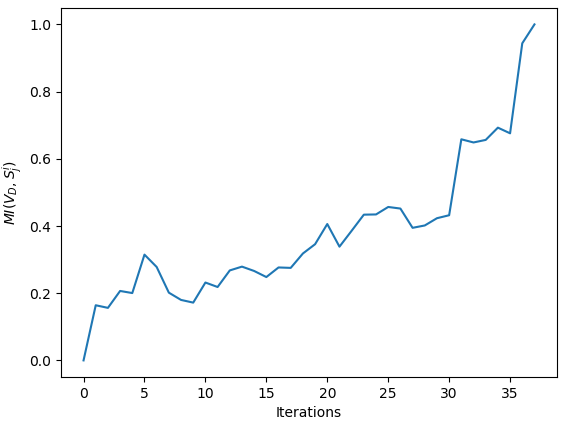
\includegraphics[width=14cm, height=6cm]{fig15}

\subsection{Stability}
Perform statistical analysis

\subsection{Initialization Time}

\end{document}

